\documentclass[a4j,dvipdfmx]{jsarticle}
\usepackage{amsmath,amssymb}

\usepackage{color}
\usepackage{ulem}
\usepackage{fancyhdr}
\usepackage{ascmac}
\usepackage{siunitx}
\usepackage[dvips]{graphicx}
\usepackage{okumacro}

\renewcommand{\thesection}{\Roman{section}}
\renewcommand{\thesubsection}{\roman{subsection}}

\begin{document}
\section*{写像ってなんすか}
「写像」...某論破王の影響で言葉事態は知っている人が多いかもしれない。ただ、その意味について考えたことはあるだろうか?
おそらくほとんどの人は「写像」の意味を知らないと思う。そこで今回はこの「写像」について学んでみよう。\xout{そして某論破王を論破しよう!}
\subsection{対応ってなんすか}
数学では、集合と並んで基本的な概念として\textbf{対応}というものがある。その定義を述べると、
\begin{screen}
    $A,B$を二つの集合とし、ある規則$\Gamma$によって$A$の各元$a$にたいしてそれぞれ一つずつ$B$の部分集合$\Gamma(a)$が定められるとする。
    そのとき、その規則$\Gamma(a)$のことを$A$から$B$の\textbf{対応}という。
\end{screen}
さらに、$A$の元$a$にたいして定まる$B$の部分集合$\Gamma(a)$を、$\Gamma$による$a$の像という。また、$A,B$をそれぞれ対応$\Gamma$の
始域(定義域)、終域という。またこのとき、$B$の部分集合のうち同じものがあってもよいし、部分集合が空集合であるような元が存在してもよい。つまり、
$\Gamma(a)=\Gamma(a')\quad(a\neq a')$であってもよいし、$\Gamma(a)=\phi$であるような$a$があってもよい。
ちなみに、$\Gamma$が$A$から$B$の対応であることを$\Gamma:A\to B$と表す。\\

とはいえ、これだけ聞いてもイメージしにくいので現実世界に置き換えて考えてみよう。\\たとえば、トマラーに友達といった時を考えてみる。
このとき、自分と知り合いを含めた客(Customer)は、お店に対してメニュー(Menu)から料理(元)を選ぶはずだ。
この客が選ぶ料理とメニューに載っている料理の関係がまさに対応である。客の集合$C$の各元はメニューの集合$M$から料理(元)を一つでも複数でも選ぶ。その選んだ品物の集合は$M$の部分集合になっているはずだ。
このとき、客ごとに選んだ料理の品はかぶってもいいし、かぶらなくてもいい。もちろん一つも料理を頼まずお冷とおしぼりだけ頼む客もいるだろう(ほんとはよくない)。
\subsection{写像ってなんすか}
さて、ここから本題の写像について考える。とはいえ写像は対応がとある性質を持つ場合のものであるため、ほとんど対応と同じみたいなものである。
その性質とは、
\begin{screen}
    $A$の任意の元$a$に対して、$f:A\to B$である対応$f$の$f(a)$は$B$のただ一つの元からなる集合である。
\end{screen}
つまり\textbf{写像}とは\underline{$A$のどんな元に対しても$B$の元を一つに対応させる}規則のことである。\\

先ほどの対応との違いは\uwave{対応先が一つの元}であるところである。そのため対応を説明する際の例は写像ではない。
逆に、我々になじみのある$f(x)=x^2$は、ある実数の集合$\mathbb{R}$の元$x$に対して実数の集合の元$x^2$が対応している
ので写像である。なお、$f(x)=x^2$のように終域が数字である場合は\textbf{関数}といい、それ以外の場合は写像ということが多い。

写像ではない例としては$x^2+y^2=1$(円の方程式)や逆三角関数がある。例えば、$\arcsin x$は$-1\leq x\leq 1$の実数$x$に対して無限個の値が存在する。
(ただ実際は主値を取っている。$\mathrm{Arcsin}\hspace{1mm}x$なら$-\frac{\pi}{2}\leq \mathrm{Arcsin}\hspace{1mm}x\leq \frac{\pi}{2}$)\\

写像$f:A\to B$によって$A$の元$a$に$B$の元$b$が対応するとき、$b$を$f$による$a$の\textbf{像}といい、
$b=f(a)$と表す。このとき、$a$を$f$による$b$の\textbf{原像}という。\xout{$a=f^{-1}(b)$と表す。}\footnote{\xout{基礎数1で習う逆関数をイメージしてみるとわかりやすい}}

\uwave{中学生でもわかること}だが、関数$f(x)=4x^2$と関数$g(x)=(2x)^2$は$\mathbb{R}$のどんな元$x$についても$f(x)=g(x)$が成り立つ。\footnote{ほかの例だとマクローリン展開とかをイメージするといい。例えば、$f(x)=e^x,g(x)=1+x+\frac{x^2}{2!}+\cdots$は一見全然違う関数に見えそうだが$f=g$である。}
同じように、$f:A\to B$である写像$f$と$g:A\to B$である写像$g$が、$A$のどんな元$a$についても常に$f(a)=g(a)$となるとき、
写像として\textbf{等しい}といい$f=g$と表す。もちろん等しくないときは$f\neq g$で表す。

\subsubsection*{問題}
$A,B$がそれぞれ$m$個,$n$個の元からなる有限集合のとき、$A$から$B$への対応は全部でいくつあるか。また、写像はいくつあるか。
{\scriptsize ヒント:まずは$A$の一つの元について考えてみよう。}
\vspace{55mm}
\subsubsection*{解答}
\color{red}
まず$A$の集合の元の一つ$a_1$について考えてみよう。このとき$A$から$B$の対応は$2^n$個ある。
なぜなら、$a_1$に対して$B$の一つの元に対応する場合は$_nC_1$個、二つの元に対応する場合は$_nC_2$個、
三つの元に対応する場合は$_nC_3$個...$n$個の元に対応する場合は$_nC_n$個あり、一つの元も対応しない場合
も合わせると
\begin{equation*}
    1+_nC_1+_nC_2+\cdots+_nC_n=2^n
\end{equation*}
となるからである。(この計算は基礎数学1問題集のstep up 464等を参照するといい.もちろん重複順列の計算(それぞれの元を対応させるさせないの2通り)でもよい.)
同様に写像についても考える。写像の場合は、一つの元$a_1$に対して$B$の元が一つ対応するわけだから、その数は$B$の元の数と同じになる。
よって$n$個。

次に、$A$のすべての元について考える。対応は$a_1$のときは$2^n$個あり、元は$a_1,a_2,\cdots,a_m$とあるわけだから、
$2^n\times 2^n\times\cdots\times 2^n=(2^n)^m=2^{mn}$となり、答えは$2^{mn}$個となる。
同様に、写像も$n\times n\times\cdots\times n=n^m$となるため、$n^m$個となる。\\\\
\rightline{\underbar{対応は$2^{mn}$個,写像は$n^m$個}}
\color{black}
\newpage
\subsection{合成写像ってなんすか}
三つの集合$A,B,C$があるときに、$A$から$C$までの写像を$B$を経由して考えることができる。
つまり、$f:A\to B\quad g:B\to C$とすると$A$から$C$までの写像は$a\in A$として$g(f(a))$となる。
これを$f,g$の\textbf{合成}または$\textbf{合成写像}$といい$g\circ f$と表す。

\subsubsection*{問5.1}
二つの写像$f:\mathbb{R}\to\mathbb{R}\quad g:\mathbb{R}\to\mathbb{R}$を$f(x)=x+2,g(x)=x^2+1$で与える。合成写像$f\circ g,\quad g\circ f\\f\circ f,\quad g\circ g$を\uwave{式で表せ}。\footnote{注意:$f(g(x))$はあくまでも像である。(合成)写像は$f\circ g$}
\vspace{30mm}

\subsubsection*{解答}
\color{red}
\begin{align*}
    f\circ g&=(x^2+1)+2=x^2+3\quad && g\circ f=(x+2)^2+1=x^2+4x+5\\
    f\circ f&=(x+2)+2=x+4\quad && g\circ g=(x^2+1)^2+1=x^4+2x^2+2\\
\end{align*}
\color{black}

次に合成写像の\textbf{結合法則}について
\begin{screen}
    写像$f:X\to Y,\quad g:Y\to Z,\quad h:Z\to W$の合成について、等式
    \begin{equation*}
        h\circ (g\circ f)=(h\circ g)\circ f
    \end{equation*}
    が成り立つ。
\end{screen}
\paragraph{証明}
各元$x\in X$に対して、
\begin{align*}
    (\text{左辺})=[h\circ (g\circ f)](x)=h((g\circ f)(x))=h(g(f(x)))\\
    (\text{右辺})=[(h\circ g)\circ f](x)=(h\circ g)(f(x))=h(g(f(x)))\\
    \therefore (\text{左辺})=(\text{右辺})\square
\end{align*} 
\newpage

\subsection{像ってなんすか}
$f:A\to B$を写像とする。$A$の部分集合$A'$に対して、$B$の部分集合$\{f(a)\mid a\in A'\}$を$f$による$A'$の\textbf{像}といい、
$f(A')$と表す。$B$の部分集合$B'$に対して、$A$の部分集合$\{a\in A \mid f(a)\in B'\}$を$f$による$B'$の\textbf{原像}または\textbf{逆像}といい、$f^{-1}(B')$と表す

\begin{figure}[h]
    \begin{minipage}{0.5\linewidth}
        \centering
        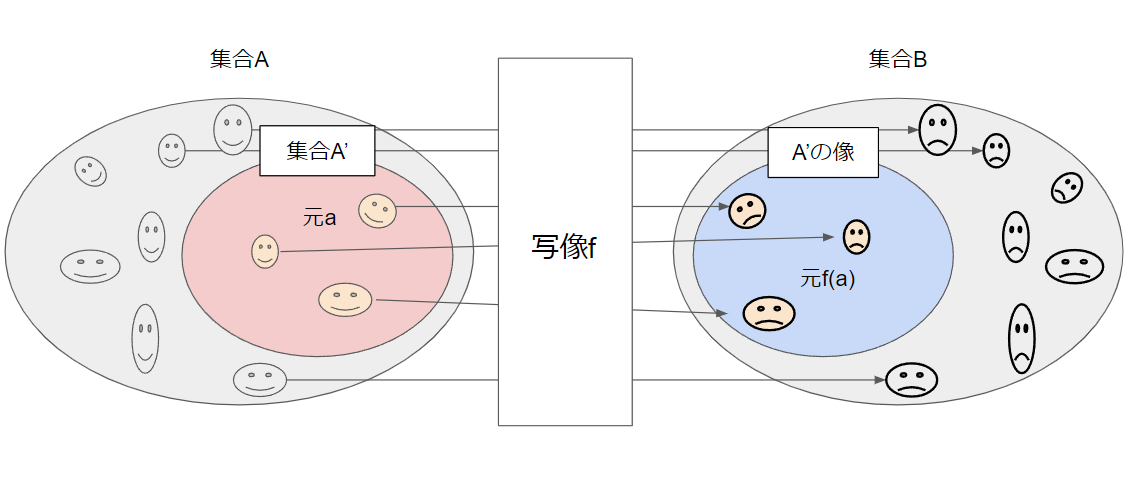
\includegraphics[keepaspectratio,scale=0.35]{img/写像_像.png}
        \caption{像のイメージ図}
      \end{minipage}
      % -- 図2--
      \begin{minipage}{0.6\linewidth}
        \centering
        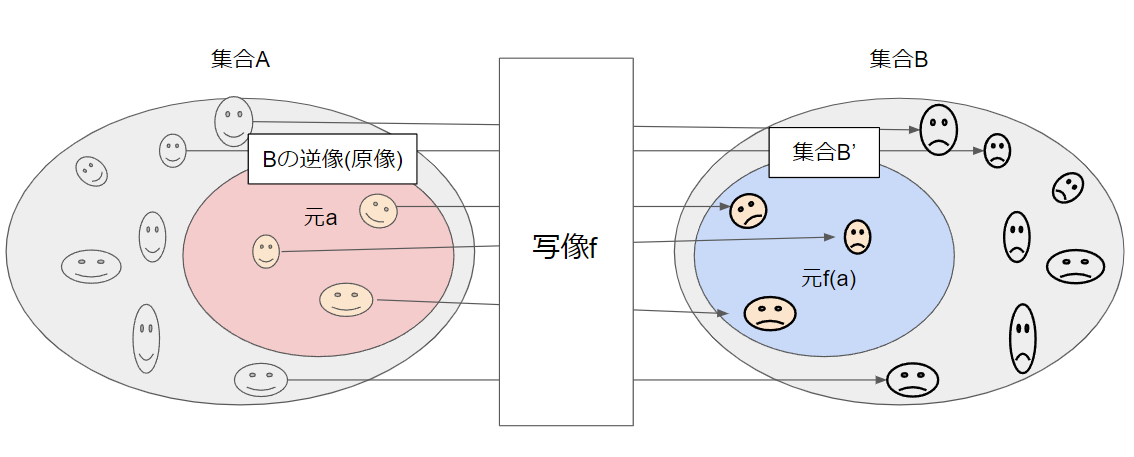
\includegraphics[keepaspectratio, scale=0.35]{img/写像_逆増.png}
        \caption{逆像のイメージ図}
      \end{minipage}
\end{figure}
\hrulefill\\
$f:A\to B$を写像とする。$A$の部分集合$A_1,A_2$および$B$の部分集合$B_1,B_2$に対して、次式が成り立つ。
\begin{align}
    f(A_1 \cup A_2)&=f(A_1)\cup f(A_2) &|& \text{$A_1$と$A_2$の和集合の像は$A_1$の像と$A_2$の像の和集合}\\
    f(A_1 \cap A_2)&\subset f(A_1)\cap f(A_2) &|& \footnotesize\text{$A_1$の像と$A_2$の像の共通部分は$A_1$と$A_2$の共通部分の像を\textbf{含む}}\\
    f^{-1}(B_1 \cup B_2)&=f^{-1}(B_1)\cup f^{-1}(B_2) &|&\\    
    f^{-1}(B_1 \cap B_2)&=f^{-1}(B_1)\cap f^{-1}(B_2) &|&\\    
    A_1 &\subset f^{-1}(f(A_1)) &|& \text{$A_1$の像の逆像は$A_1$を\textbf{含む}}\\
    f(f^{-1}(B_1)) &\subset B_1 &|&\\
    f(A_1)-f(A_2) &\subset f(A_1-A_2) &|&\text{\small※差集合$A-B$は\textbf{$A$に含まれて$B$に含まれない}元の集合}\\
    f^{-1}(B_1)-f^{-1}(B_2) &= f^{-1}(B_1-B_2) &|&
\end{align}
図でイメージするとなんとなくのイメージはつかみやすいかもしれない。

とはいえ、ただ式を並べただけでは「なんかそういうデータってあるんすか?」と言われてしまうので、簡単に証明もしておこう。

\paragraph{証明}
まずは、(1)を証明する。このページの本文の一行目から二行目に書いてあることをそのまま用いる。

\begin{align*}
    f(A_1\cup A_2)
    &=\left\{f(a)\mid a\in A_1\cup A_2 \right\}\\
    &=\left\{f(a)\mid a\in A_1\text{または} a\in A_2 \right\}\\
    &=f(A_1)\cup f(A_2)\quad\square
\end{align*}

% 左辺の$f(A_1\cup A_2)$は、$\left\{b\in B\mid \text{$b=f(a)$となる元$a\in A_1 \cup A_2$が存在する}\right\}$と書ける。なぜなら、\\
% $f$は$A\to B$の写像だからこの集合の元は必ず$B$の元となるはずであり、さらに写像の定義\footnote{$A$のどんな元も$B$の元を一つに対応させる規則}とかっこの中身から\uwave{$b=f(a)\quad (a\in A_1\cup A_2)$を満たす$a$が存在する}ことが条件であるからである。

% ここで下線部の条件は$A_1\cup A_2$から\\
% $\left\{b\in B\mid \text{\underbar{$b=f(a_1)$となる元$a_1\in A_1$}または$b=f(a_2)$となる元$a_2\in A_2$が存在する}\right\}$\\と言い換えられる。
% 次に下線部のところに着目するとこれは$b\in f(A_1)$と書き換えられる。\footnote{このページの一行目を参照}「または...」以降も同様に書き換えると、
% $\left\{b\in B\mid b\in f(A_1)\text{または} b\in f(A_2)\right\}$となる。これはまさに右辺の式そのものとなる。$\square$
% \newpage
% (1)の証明を式で書くと次のようになる。
% \begin{align*}
%     f(A_1\cup A_2)&=\left\{b\in B\mid \text{$b=f(a)$となる元$a\in A_1 \cup A_2$が存在する}\right\}\\
%     &=\left\{b\in B\mid \text{$b=f(a_1)$となる元$a_1\in A_1$または$b=f(a_2)$となる元$a_2\in A_2$が存在する}\right\}\\
%     &=\left\{b\in B\mid b\in f(A_1)\text{または} b\in f(A_2)\right\}\\
%     &=f(A_1)\cup f(A_2).
% \end{align*}
% 通してみてみると意外とあっけない。\\

次に(2)を証明する。こちらも(1)とちがい、後の都合上$f(A_1\cap A_2)$を$$\left\{b\in B\mid \text{$b=f(a)$となる元$a\in A_1 \cap A_2$が存在する}\right\}$$と書く(書ける)。
左の「~が存在する」という条件を満たす時の$b$のみが入っているのは定義をそのまま書いたようなものだ。(存在しないときはその$b$は集合にいれない)\\
この次がポイントでこの集合は\\
$\left\{b\in B\mid \text{$b=f(a_1)$となる元$a_1\in A_1$および$b=f(a_2)$となる元$a_2 \in A_2$が存在する}\right\}$\\
に\textbf{含まれている}といえる。

なぜなら、この条件「$b=f(a_1)$となる$a_1\in A_1$および$b=f(a_2)$となる$a_2\in A_2$が存在する」は
\textbf{$A_1$に含まれる元}の条件と\textbf{$A_2$に含まれる元}の条件であるのに対し、最初の条件は$A_1\cap A_2$に含まれる元の条件
となっており、元が含まれる\ruby{元}{もと}の集合は明らかに前者のほうが大きいためである。おそらく何言ってるかわからないと思うので例を出すと、
$A_1$と$A_2$の対称差\footnote{$A_1$のみの元の集合と$A_2$のみの元の集合の和集合}の元は、始めの条件の適応外であるが後の条件の範囲内である。\\
さらにこの条件は、$\left\{b\in B\mid b\in f(A_1)\text{かつ}b\in f(A_2)\right\}$と書き換えられるので、右辺の式そのものとなる。$\square$

これも、式で書くと次のようになる。
\begin{align*}
    f(A_1\cap A_2)&=\left\{b\in B\mid \text{$b=f(a)$となる元$a\in A_1 \cap A_2$が存在する}\right\}\\
    &\subset\left\{b\in B\mid \text{$b=f(a_1)$となる元$a_1\in A_1$および$b=f(a_2)$となる元$a_2 \in A_2$が存在する}\right\}\\
    &=\left\{b\in B\mid b\in f(A_1)\text{かつ} b\in f(A_2)\right\}\\
    &=f(A_1)\cap f(A_2).\\
    \therefore f(A_1\cap A_2)&\subset f(A_1)\cap f(A_2).
\end{align*}
(1)に比べて難しかったと思う。「なぜなら...」のところは図を書いてみると分かりやすいかもしれない。

次は(3)を証明する。これも前ページの定義をそのまま用いればよい。
\begin{align*}
    f^{-1}(B_1\cup B_2)
    &=\left\{a\in A\mid f(a)\in B_1\cup B_2\right\}\\
    &=\left\{a\in A\mid f(a)\in B_1 \text{または}f(a)\in B_2\right\}\\
    &=f^{-1}(B_1)\cup f^{-1}(B_2)\square
\end{align*}
\hrulefill\\
(4)は省略する。演習問題で解く。\\
\hrulefill

つづいて(5)を証明する。\\
定義より、$a\in A_1$ならば$f(a)\in f(A_1)$である。このとき原像の定義から$$f^{-1}(f(A_1))=\left\{a\in A\mid f(a)\in f(A_1)\right\}=\left\{a\in A_1\right\}\cup\left\{a\in A-A_1\mid f(a)\in f(A_1)\right\}$$
となるため、$A_1\subset f^{-1}(f(A_1))$が成り立つ。$\square$

例えば、$A=\mathbb{R},A_1=\{1,2\}\subset\mathbb{R}$とし、$f:\mathbb{R}\to\mathbb{R}$となる写像$f$を考える。この時この写像を$f(x)=x^2$という式で与えたとする。
そうすると$f(A_1)=\{1,4\}$となる。ではここで$f^{-1}(f(A_1))$を考えると、これは$\{-2,1,1,2\}$となり、この中に$A_1=\{1,2\}$が含まれているのがわかる。\\

つぎは(6)を証明する。まず$b\in f(f^{-1}(B_1))$とする。この時右辺は、
$$f(f^{-1}(B_1))=\left\{x\in B\mid x=f(a)となるa\in f^{-1}(B_1)が存在する\right\}$$
であり、仮定より「$b=f(a)$となる元$a\in f^{-1}(B_1)$が存在する」といえる。ここで、原像の定義から$a\in f^{-1}(B_1)$と
$f(a)\in B_1$が同値であること\footnote{集合の条件に注目}に気づけば、直ちに$b=f(a)\in B_1$とわかる。よって、$f(f^{-1}(B_1))\subset B_1$が成り立つ。$\square$
\newpage
では最後に(7)を証明する。差集合の定義から
\begin{align*}
    f(A_1)-f(A_2)
    &=\left\{b\in B\mid b\in f(A_1)\text{かつ}b\notin f(A_2)\right\}\\
    &=\left\{b\in B\mid b=f(a)\text{となる元$a\in A_1$が存在し、かつ}b\notin f(A_2)\right\}\\
    &\subset \left\{b\in B\mid b=f(a)\text{となる元$a\in A_1-A_2$が存在する}\right\}\\
    &=f(A_1-A_2)
\end{align*}
三番目の式は、$A_1$と$A_2$の共通部分があるときは\textbf{等号}になる。

これも例を見てイメージしよう。例えば、$A_1=\{1,2,3\}\subset\mathbb{R},A_2=\{1,2\}\subset\mathbb{R}$とし、$f:\mathbb{R}\to\mathbb{R}$となる写像$f$を考える。この時この写像を$f(x)=x^2$という式で与えたとする。
そうすると$f(A_1)-f(A_2)=\{9\}$となり、これは$f(A_1-A_2)$に等しい。ではここで共通部分をなくして$A_2=\{-1,-5\}$を考えると、$f(A_1)-f(A_2)=\{4,9\}$となり、$f(A_1-A_2)=\{1,4,9,25\}$と比べると明らかに$f(A_1-A_2)$に含まれていることがわかる。\\
\hrulefill\\
(8)は省略する。演習問題で解く。\\
\hrulefill

\subsubsection*{問題}
$f(x)=x^2$によって写像$f:\mathbb{R}\to\mathbb{R}$を定める。$\mathbb{R}$の部分集合$A_1,A_2,B_1$として、閉区間
\begin{equation*}
    A_1=[-3,1]\quad A_2=[-1,2]\quad B_1=[-1,1] 
\end{equation*}
を定める。この時、$f(A_1\cap A_2)=[0,1]\quad\because A_1\cap A_2=[-1,1]$である。
これに倣い、以下の像・原像を求めよ。
\begin{align*}
    f(A_1)\cap f(A_2)\qquad f^{-1}(f(A_1))\qquad f(f^{-1}(B_1))\qquad f(A_1)-f(A_2)\qquad f(A_1-A_2)
\end{align*}
\vspace{3cm}
\subsubsection*{解答}
\color{red}
$f(A_1)=[0,9]\quad f(A_2)=[0,4]\quad A_1-A_2=(-1,-3]$より、
\begin{alignat*}{2}
    & f(A_1)\cap f(A_2) & = &[1,4]\qquad, f^{-1}(f(A_1))=[-3,3]\\
    & f(f^{-1}(B_1)) & = &f([0,1]\text{または}[-1,0])=[0,1]\\
    & f(A_1)-f(A_2) & = & (4,9]\qquad,f(A_1-A_2)=(1,9]
\end{alignat*}
となる。このことから先ほどの(2),(5),(6),(7)は一般には等号が成り立たないことがわかる。
\color{black}
\newpage
\subsubsection*{問題}
(4),(8)を証明せよ。
\vspace{10cm}
\subsubsection*{解答}
\color{red}
(4)の証明。原像の定義より、
\begin{align*}
    f^{-1}(B_1\cap B_2)
    &=\left\{a\in A\mid f(a)\in B_1\cap B_2\right\}\\
    &=\left\{a\in A\mid f(a)\in B_1\text{かつ} f(a)\in B_2\right\}\\
    &=f^{-1}(B_1)\cap f^{-1}(B_2)\square
\end{align*}

(8)の証明。差集合の定義から
\begin{align*}
    f^{-1}(B_1)-f^{-1}(B_2)
    &=\left\{a\in A\mid a\in f^{-1}(B_1) \text{かつ} a\notin f^{-1}(B_2)\right\}\\
    &=\left\{a\in A\mid f(a)\in B_1 \text{かつ} f(a)\notin B_2\right\}\\
    &=\left\{a\in A\mid f(a)\in B_1-B_2\right\}\\
    &=f^{-1}(B_1-B_2)\square
\end{align*}
\color{black}
\hrulefill\\
7/02 以下はまだ書き終えていないです。
\newpage
\subsection{集合系の演算}


\end{document}